\documentclass[a4paper, oneside, 11pt]{memoir}
\usepackage[margin=1in]{geometry}
\usepackage[inline]{enumitem}
\usepackage{color}
\usepackage{tikz}
\usetikzlibrary{arrows,shapes,positioning,shadows,trees}
\tikzset{
  basic/.style  = {draw, text width=2cm, drop shadow, font=\sffamily, rectangle},
  root/.style   = {basic, rounded corners=2pt, thin, align=center,
                   fill=green!30},
  level 2/.style = {basic, rounded corners=6pt, thin,align=center, fill=green!60,
                   text width=8em},
  level 3/.style = {basic, thin, align=left, fill=pink!60, text width=10.5em}
}

\renewcommand{\baselinestretch}{1.15}

%%%%%%%%%%%%%%%%%%%%%%%%%%%%%%%%%%%%%%%%%%%%%Timeline%%%%%%%%%%%%
\usepackage[margin=3cm]{geometry}
\usepackage{ragged2e}
\usepackage{fourier}
\usepackage{tikz} 
\usetikzlibrary{chains,shapes.arrows,fit}

\definecolor{arrowcolor}{RGB}{201,216,232}% color for the arrow filling
\definecolor{circlecolor}{RGB}{79,129,189}% color for the inner circles filling
\colorlet{textcolor}{white}% color for the text inside the circles
\colorlet{bordercolor}{white}% color for the outer border of circles

\pgfdeclarelayer{background}
\pgfsetlayers{background,main}

\newcounter{task}

\newlength\taskwidth% width of the box for the task description
\newlength\taskvsep% vertical distance between the task description and arrow

\setlength\taskwidth{2.5cm}
\setlength\taskvsep{17pt}

\def\taskpos{}
\def\taskanchor{}

\newcommand\task[1]{%
  {\parbox[t]{\taskwidth}{\scriptsize\Centering#1}}}

\tikzset{
inner/.style={
  on chain,
  circle,
  inner sep=4pt,
  fill=circlecolor,
  line width=1.5pt,
  draw=bordercolor,
  text width=1.2em,
  align=center,
  text height=1.25ex,
  text depth=0ex
},
on grid
}

\newcommand\Task[2][]{%
\node[inner xsep=0pt] (c1) {\phantom{A}};
\stepcounter{task}
\ifodd\thetask\relax
  \renewcommand\taskpos{\taskvsep}\renewcommand\taskanchor{south}
\else
  \renewcommand\taskpos{-\taskvsep}\renewcommand\taskanchor{north}
\fi
\node[inner,font=\footnotesize\sffamily\color{textcolor}]    
  (c\the\numexpr\value{task}+1\relax) {#1};
\node[anchor=\taskanchor,yshift=\taskpos] 
  at (c\the\numexpr\value{task}+1\relax) {\task{#2}};
}

\newcommand\drawarrow{% the arrow is placed in the background layer 
                                                     % after the node for the tasks have been placed
\ifnum\thetask=0\relax
  \node[on chain] (c1) {}; % if no \Task command is used, the arrow will be drawn
\fi
\node[on chain] (f) {};
\begin{pgfonlayer}{background}
\node[
  inner sep=10pt,
  single arrow,
  single arrow head extend=0.8cm,
  draw=none,
  fill=arrowcolor,
  fit= (c1) (f)
] (arrow) {};
\fill[white] % the decoration at the tail of the arrow
  (arrow.before tail) -- (c1|-arrow.west) -- (arrow.after tail) -- cycle;
\end{pgfonlayer}
}

\newenvironment{timeline}[1][node distance=.75\taskwidth]
  {\par\noindent\begin{tikzpicture}[start chain,#1]}
  {\drawarrow\end{tikzpicture}\par}
%%%%%%%%%%%%%%%%%%%%%%%%%%%%%%%%%%%%%%%%%%%%%%%%%%%%%%%%%%%%%%%%%
\usepackage{pdfpages}
\usepackage{graphicx}
\title{Decouple Yet Control}
\author{Amit Kumar Singh}
\begin{document}
\maketitle
\pagebreak
\renewcommand{\abstractname}{Executive Summary}
\begin{abstract}
\textbf{Short term action plan:}conduct recurring meetings with Venkat to reach \textbf{mutual agreement}. The agreement would list the top three concerns inhibiting compliance with IWAY. \textbf{Finer point:}The process of mutual agreement must be based on mutual respect \cite{smeltzer1997meaning} and it must be founded on the ideas of Authoritative, Affiliative and Democratic style of leadership \cite{goleman2000leadership} to nudge \cite{leonard2008richard} Venkat into compliance. \cite{tittle2018control} \cite{inderst2011countervailing} \\\textbf{Long term strategy:} IWAY policies and practices should be revised to work with consortiums to neutralize threat to IKEA's value chain.\footnote{ from hostile organizations that deploy intended and organized attacks.} \cite{publichearing1998_183}\\
There are \textbf{three main benefits} of redefined relationship between IKEA and its suppliers - \\
\begin{enumerate*}
 \item \textbf{Brand-Image Improved}\footnote{Competitive advantage by forward integration: by appealing to customer's sentiments} ,
 \item \textbf{Cost Savings Improved}\footnote{Competitive advantage by backward integration : by increase in IKEA's control-surface on supplier's business processes},
 \item \textbf{Improved management of risks}\footnote{Sustainability and Collaborative advantage: associated with environmental and social resources.}
\end{enumerate*} \\
Three main concerns that can be raised are - \\
\begin{enumerate*}
 \item \textbf{New cost} to meet the requirements of strict compliance.\footnote{ requires exhaustive monitoring, which is expensive in many dimensions. Because, compliance is difficult to validate in the real world. I present a supporting quote from a recent research - "central premise is that the total amount of control people are subjected to, relative to the control they can exercise, will affect the probability and type of their deviant behavior." }\footnote{tighter coupling of business models is not recommended. This is against the fundamental  principles of system architecture.}\cite{tittle2018control}
 \item \textbf{Threat to sales:} misalignment of IKEA's goals with those of the media that influences customers would affect IKEA's business. 
 \item \textbf{Accounting liability:}IKEA's business model is tightly coupled with geopolitical dynamics. This is a huge accounting liability in terms of potential litigations.
\end{enumerate*}
\end{abstract}

\section{Reasoning}
\begin{enumerate*}
\item To ensure \textbf{better yet cost effective IWAY compliance}, intensity of supplier-monitoring must not scale proportional to IKEA's sales. \textbf{Scale and complexity of IKEA's supplier base as a whole is directly proportional to IKEA's sales}. IKEA should \textbf{aim to decouple from complexity of its suppliers to keep cost of monitoring independent}. One practical solution to mitigate the proportional rise of cost is to \textbf{collaborate with local organizations that understand local socioeconomic structure}. This reasoning feeds into short time actions that IKEA must undertake.
\item In order to mitigate threat to sales, IKEA works with other organizations like - "Swedish Work Group for Abolishment of Child Labour in the Carpet Industry", "Swedish Save the children", and "International Labour Organisation"\cite{publichearing1998_479}. IKEA must actively collaborate with the activism groups in Sweden and those that operate at international organizations. This will ensure competitive advantage by forward integration \cite{harrigan1985vertical}. This reasoning feeds into long term strategy along with the next and final point.
\item IKEA must look at IWAY as a control system that evolves with appropriate deployment of a feedback from geopolitical events.
\end{enumerate*}


\section{Appendix A}

I present a timeline in "Figure 1", which shows chronological events in the case. I also show the \%-change in sales YoY (in "Figure 2"). 

By observing these diagrams in juxtaposition one can observe relationship between the geopolitical events mentioned in the timeline and dip in \%-change in sales. Between the years 1995 to year 2000 large amount of change in sales is observed and during the same time frame, as observed in the timeline from circle marked to that marked 6, one can observe negative coverage in media were reported. This shows the interdependence of consumer perception of a brand, the media agencies that influence this perception and phenomenon that how these factors interact with a business's performance. \\
\subsection{Timeline}
Figure 1: The Chronology of Events for IKEA's Child-Labor Ordeal \\

\begin{timeline}
\Task[1]{\textbf{Seed:Child Labor Deterrent Act} was proposed for debate in U.S. Congress\\\textbf{Year 1993} }
\Task[1.1]{\textbf{Unintended Consequences}}
\Task[2]{\textbf{Problem:}First report of Child Labor\\\textbf{Mitigation}\\Strategy:International Labor Organization (ILO)\\\textbf{Year 1994}}
\Task[2.1]{\textbf{Unintended Consequences 2} Induced unemployment in Pakistan}
\Task[3]{\textbf{Problem:}Monitoring was impractical\\\textbf{Scale and Nature of Manufacturing Process}\\\textbf{Fall 1994}}
\Task[4]{\textbf{May 1995}\\\textbf{Problem:}Investigative Report of Child Labor\\\textbf{Mitigation}\\Evidence:Report found fabricated}
\Task[5]{\textbf{Year 1998}\\Marianne Barner becomes IKEA\textquotesingle s children\textquotesingle s ombudsman}
\end{timeline}

\begin{timeline}
\Task[6]{\textbf{1998-99} 10-day educational tours of India\\ for IKEA's retail managers from different countries}
\Task[7]{\textbf{2004} registered success of joint program by UNICEF and IKEA\\ with ACL and Self-Help groups programs}
\Task[7.1]{\textbf{2004} IKEA terminated 10 supplier relationships for violations of its IWAY Code}
\Task[8]{\textbf{2005} Dahlvig's \textbf{10 Jobs for 10 Years} document released}
\end{timeline}

Figure 2:\%-Change in Sales\\

\begin{figure}[h]
   \centering
   \begin{tabular}{c}
       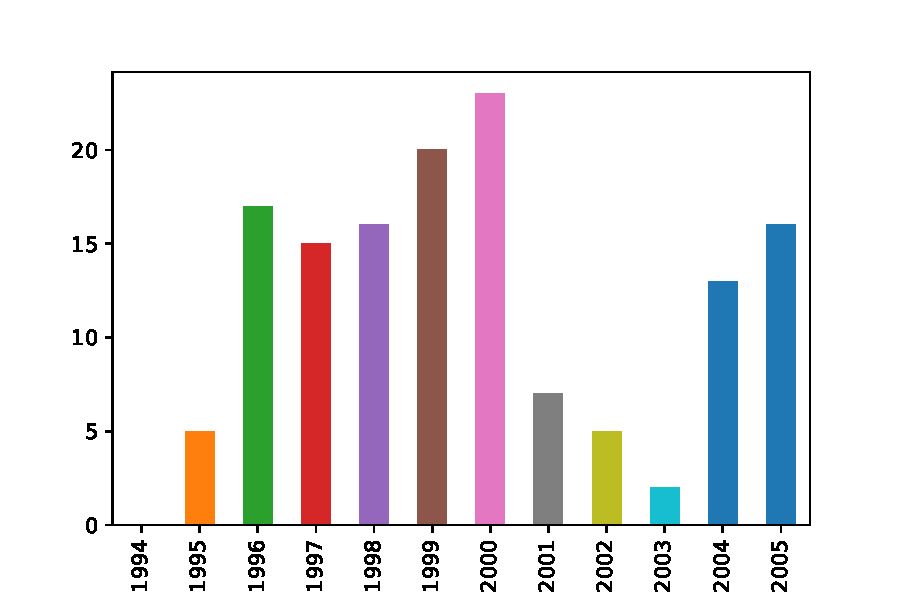
\includegraphics[page=1,width=.9\textwidth]{fig2.pdf} \\
   \end{tabular}
\end{figure}

%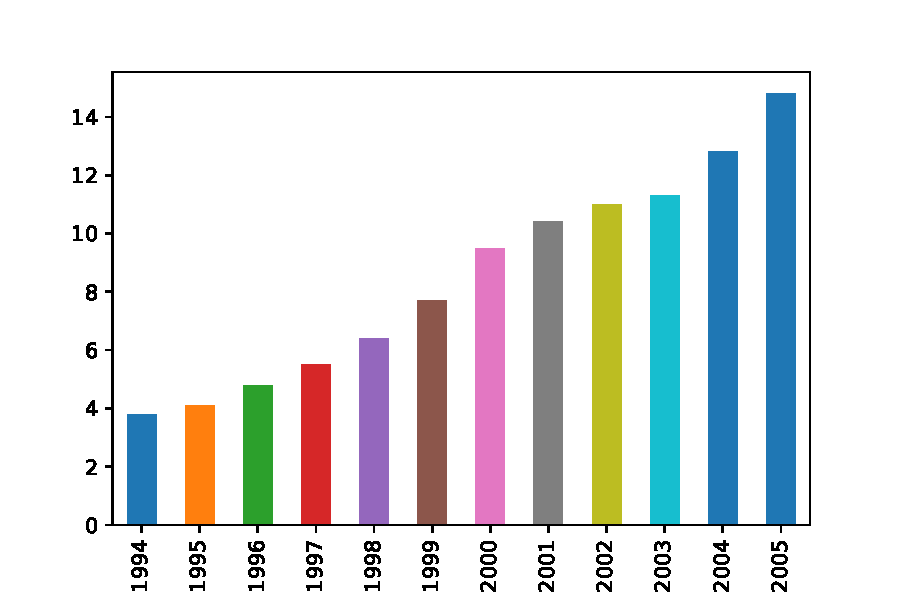
\includepdf{fig.pdf}
%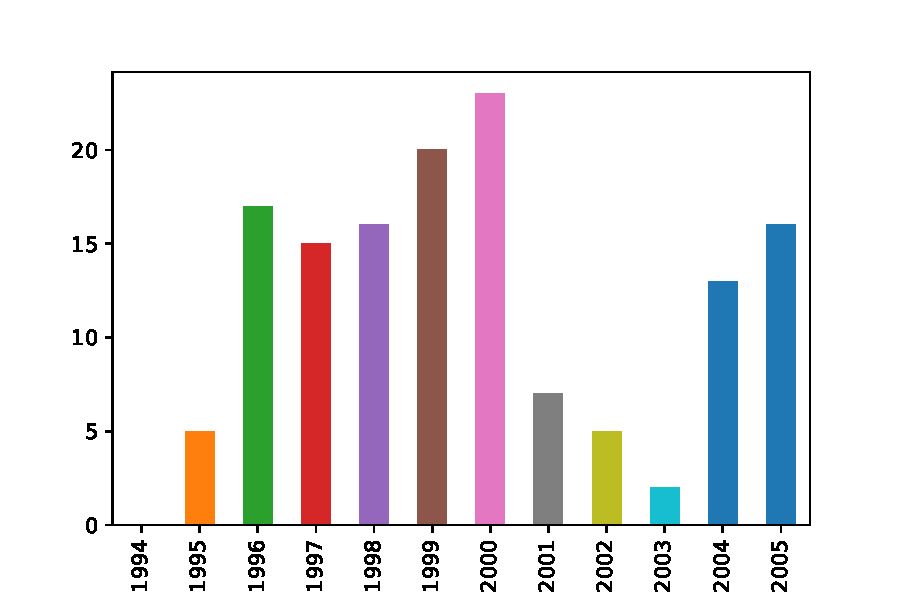
\includepdf{fig2.pdf}
\section{Situation/Complications/Questions}
Here's a short summary of the case:\\
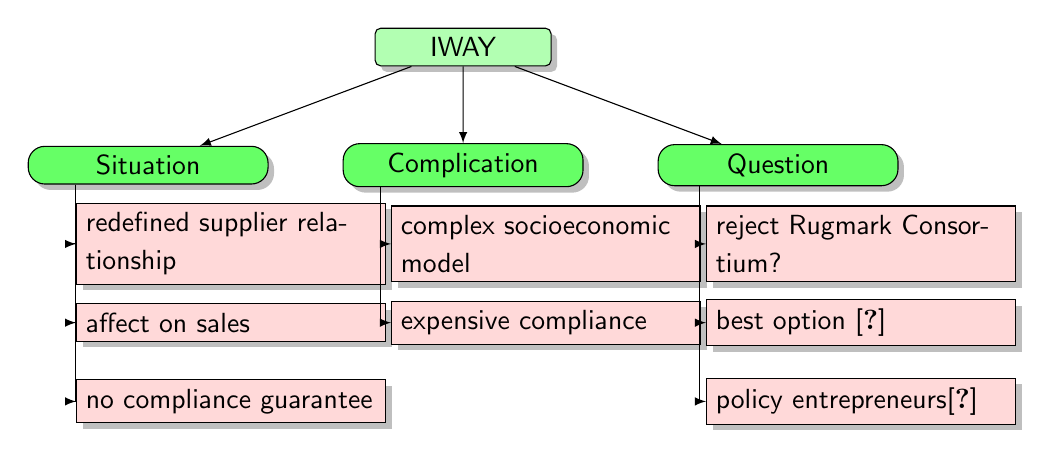
\begin{tikzpicture}[
  level 1/.style={sibling distance=40mm},
  edge from parent/.style={->,draw},
  >=latex]

% root of the the initial tree, level 1
\node[root] {IWAY}
% The first level, as children of the initial tree
  child {node[level 2] (c1) {Situation}}
  child {node[level 2] (c2) {Complication}}
  child {node[level 2] (c3) {Question}};

% The second level, relatively positioned nodes
\begin{scope}[every node/.style={level 3}]
\node [below of = c1, xshift=30pt] (c11) {redefined supplier relationship};
\node [below of = c11] (c12) {affect on sales};
\node [below of = c12] (c13) {no compliance guarantee};

\node [below of = c2, xshift=30pt] (c21) {complex socioeconomic model};
\node [below of = c21] (c22) {expensive compliance};

\node [below of = c3, xshift=30pt] (c31) {reject Rugmark Consortium?};
\node [below of = c31] (c32) {best option \cite{publichearing1998_183}};
\node [below of = c32] (c33) {policy entrepreneurs\cite{anderson2018policy}};
\end{scope}

% lines from each level 1 node to every one of its "children"
\foreach \value in {1,2,3}
  \draw[->] (c1.195) |- (c1\value.west);

\foreach \value in {1,...,2}
  \draw[->] (c2.195) |- (c2\value.west);

\foreach \value in {1,...,3}
  \draw[->] (c3.195) |- (c3\value.west);
\end{tikzpicture}

 %\footnote{I present this statement from a research done in 2018 - "..the success or failure of early nineteenth-century child labor laws depended on these actors’ social skill, pragmatic creativity, and goal-directedness." \cite{anderson2018policy} Here "actors" refers to "elite policy entrepreneurs".} 
  
\begin{thebibliography}{9}
    \bibitem{goleman2000leadership}
    Goleman, D. (2000). Leadership that gets results. Harvard business review, 78(2), 4-17.
    \bibitem{leonard2008richard}
    Leonard, T. C. (2008). Richard H. Thaler, Cass R. Sunstein, Nudge: Improving decisions about health, wealth, and happiness.
    \bibitem{tittle2018control}
    Tittle, C. R. (2018). Control balance: Toward a general theory of deviance. Routledge.
    \bibitem{anderson2018policy}
    Anderson, E. (2018). Policy Entrepreneurs and the Origins of the Regulatory Welfare State: Child Labor Reform in Nineteenth-Century Europe. American Sociological Review, 83(1), 173-211.
    \bibitem{publichearing1998_183}
    United States. International Child Labor Program. (1998). Public hearings on international child labor. United States:Page:183
    \bibitem{publichearing1998_479}
    United States. International Child Labor Program. (1998). Public hearings on international child labor. United States:Page:479
    \bibitem{smeltzer1997meaning}
    Smeltzer, L. R. (1997). The meaning and origin of trust in buyer‐supplier relationships. International journal of purchasing and materials management, 33(4), 40-48.
    \bibitem{inderst2011countervailing}
    Inderst, R., \& Wey, C. (2011). Countervailing power and dynamic efficiency. Journal of the European Economic Association, 9(4), 702-720.
    \bibitem{harrigan1985vertical}
    Harrigan, K. R. (1985). Vertical integration and corporate strategy. Academy of Management journal, 28(2), 397-425.
\end{thebibliography}
\end{document}